\section{Additional Data}
\subsection{Comparison of Setup-schemes}
\label{app:CompSetup}
Moreover, the library \prog{tetgen} \cite{tetgen} used to construct the meshes also may vary the point-distribution locally by adding additional points to ensure high quality tetrahedra, \textit{i.e.} the ratio of its circumsphere and the shortest edge is bounded in all results presented in this work by $1.5$ and the maximum volume of any tetraheder is below $8\,$bohr$^3$ whereby the latter has only minor influence on the mesh \cite{tetgen}.
To compare the resulting meshes, in Table \ref{tab:RadScheme} some characteristics of the results obtained for an atomic mesh (\textit{i.e.} using only one sphere) are presented, using a Lebedev-grid \cite{lebedev} for the spherical distribution.
As radial distribution, the tm-mapping \eq{eq:tm_map} is used for the schemes denoted as \textit{const} and \textit{tm} whereas \eq{eq:son_map}) map is used for the scheme \textit{son}.
The number of points per sphere is $M_i=74$ for all spheres for the \textit{const} scheme and according to \eq{eq:tm_num} and \eq{eq:son_num} for the others, respectively.
The parameters for the radial mapping are chosen as $q=1.8$ and $p=2.6$.
\begin{table}
\begin{tabular}{|c|c|c|c|}
\hline
scheme & runtime [s] & DOS$^{a)}$ [$(m E_h)^{-1}$] & number of nodes\\
\hline
const   &  438   &    7    &   3255 \\
tm      &  825   &    13   &   5132 \\
son     &  891   &    4    &   6368 \\
\hline
\end{tabular}
%\caption{The runtime, density of states and number of nodes used for the different radial mapping schemes that are described in the text.\\
\caption{ Different properties of the solutions obtained with different setup-schemes as described in the text.\\
$^{a)}$: density of states (eigenenergies), averaged over 23 states}
\label{tab:RadScheme}
\end{table}
Some characteristic properties of the respective results are shown in Table \ref{tab:RadScheme}.
%The runtime given in this table is only a rough estimation but seem to scale directly proportional to the number of nodes.
The main conclusion to be drawn from Table \ref{tab:RadScheme} is that the density of states is much larger for the radial mapping scheme suggested here compared to the son scheme.
It should be noted, however, that the direct comparison of the schemes is disputable due to the different dependence on the parameter $q$ and thus a more detailed study would be needed to draw definite conclusions about the quality of the schemes.
Moreover, the density of eigenenergies is not uniform along the spectrum and thus can depend on the number of states taken into account.
Finally, also the adaption of the mesh to ensure a good quality of the tetrahedra has some influence here.
%Moreover, during the creation of tetrahedra from the given point-sets a quality-check is done by the respective library \cite{tetgen} which adds or removes points to ensure well-shaped tetrahedra which may, however, alter the distributions considerably.
\begin{figure}
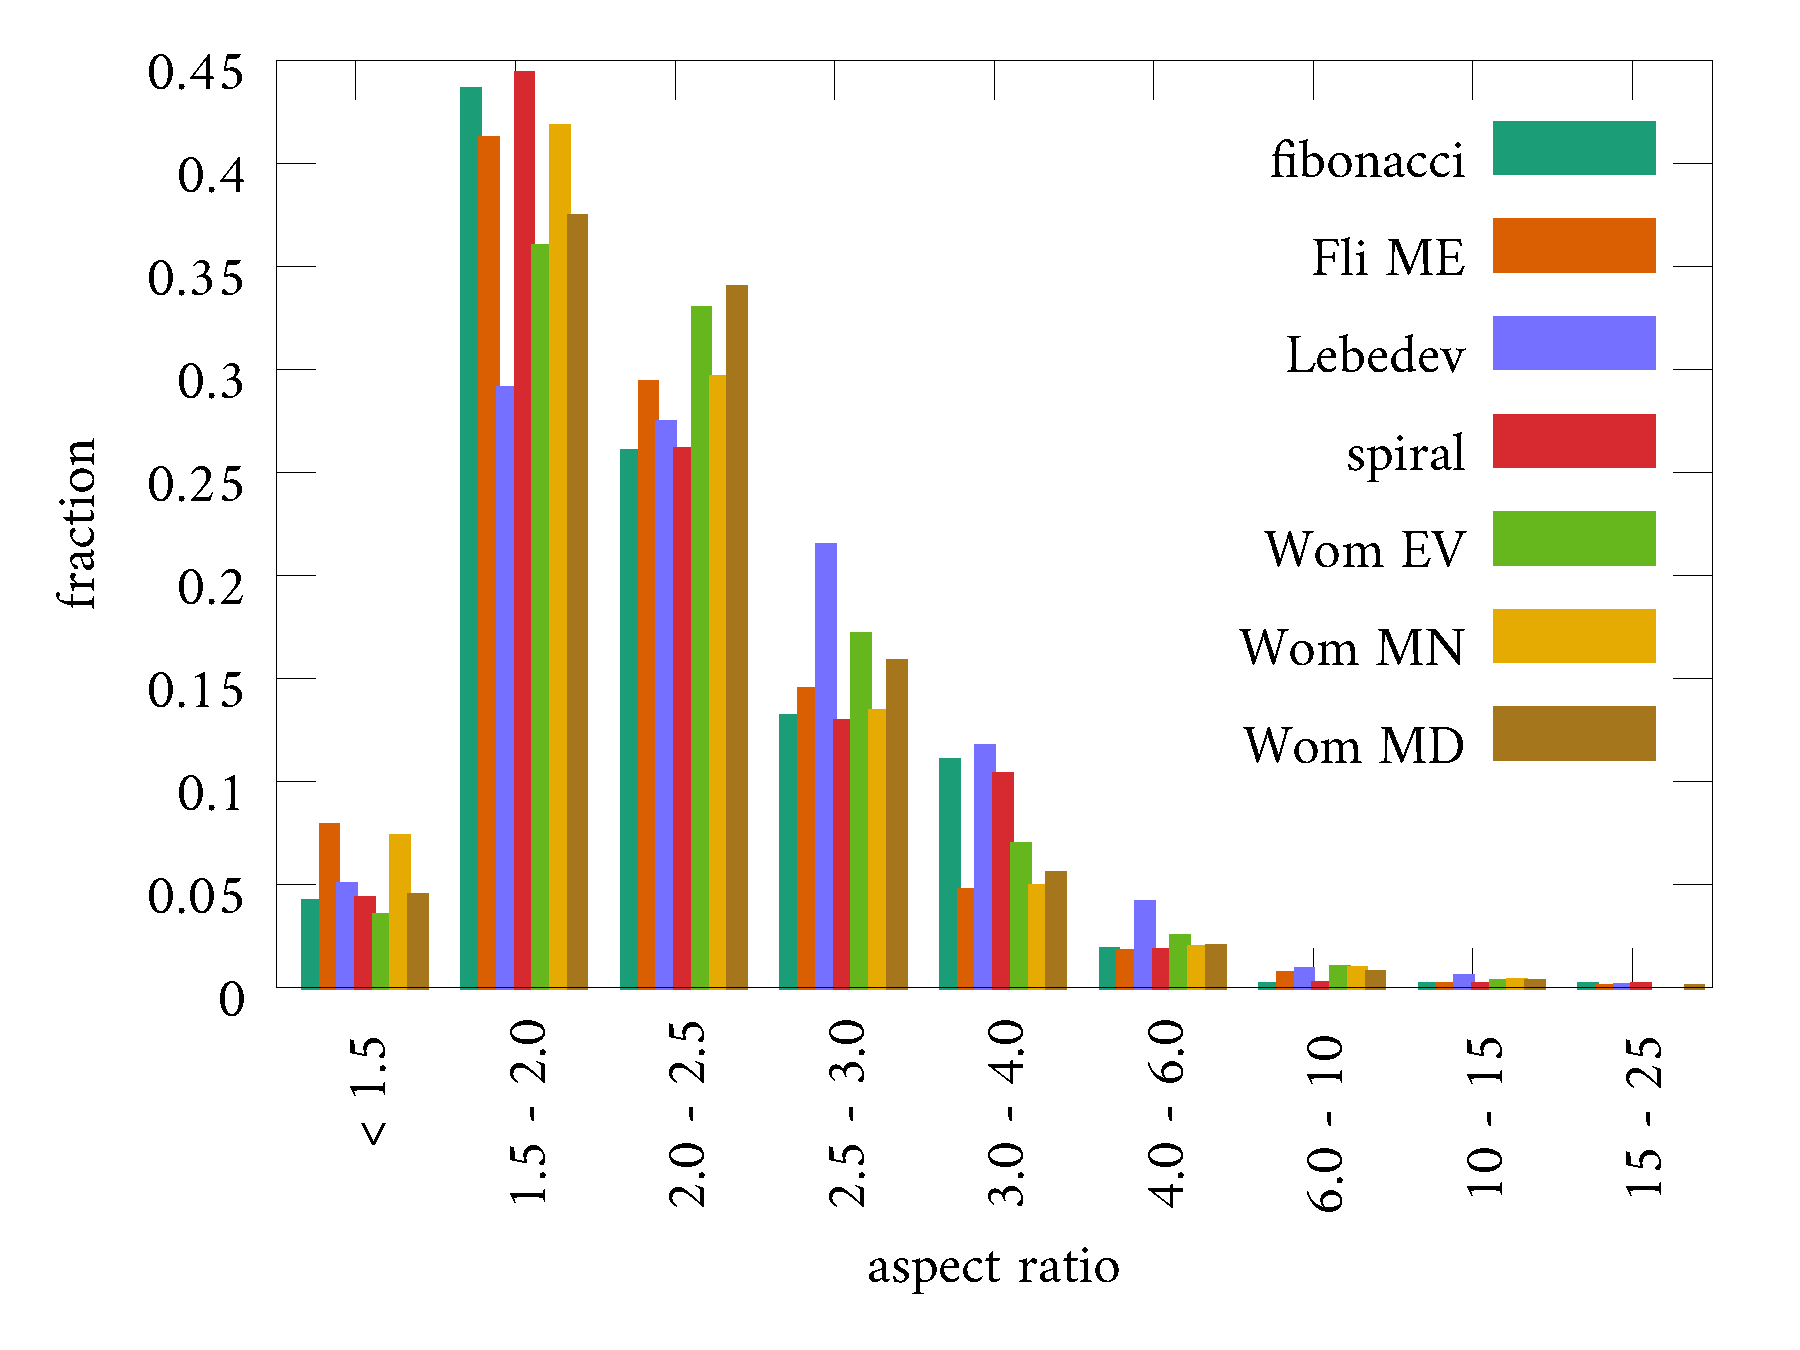
\includegraphics[width=0.49\textwidth]{Figures/Sph_hist.pdf}
\caption{Distribution of aspect ratio (longest edge length divided by the smallest side height).
   Be aware that the ranges of the different bins differ.}
\end{figure}

To illustrate the very similar statistics obtained by the different mapping schemes described and discussed in section \ref{ch:GridSetup}, in Figure \ref{appFig:SchemHist} further properties are shown, each normalised for better comparatibility.
In the figures, the radius-edge ratio denotes the ratio of the radius of circumsphere divided by the sortest edge length.
\begin{figure}
\begin{subfigure}{0.5\textwidth}
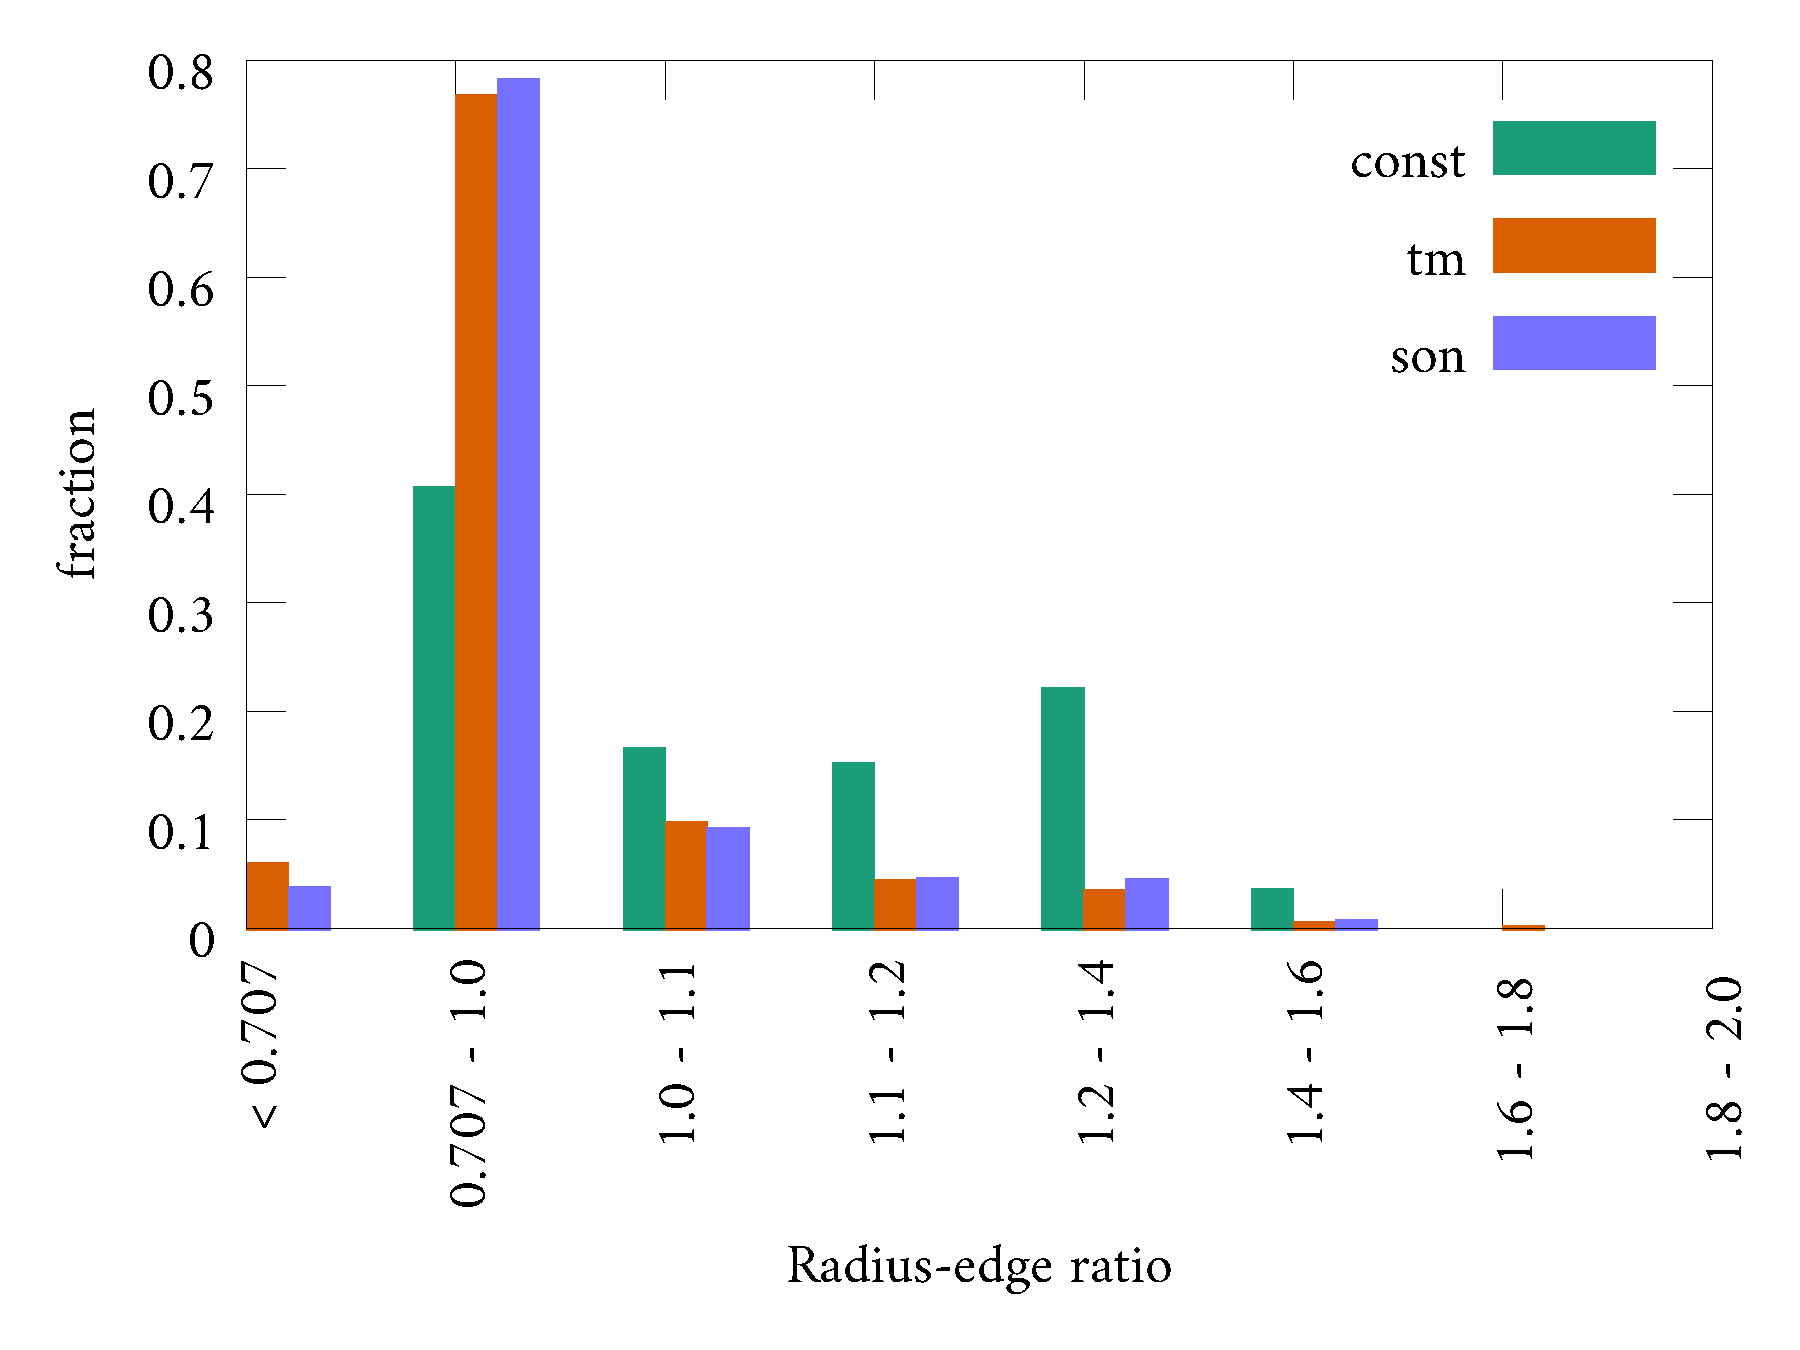
\includegraphics[width=\textwidth]{Figures/App/Rad_histAp1.pdf}
\end{subfigure}
\begin{subfigure}{0.5\textwidth}
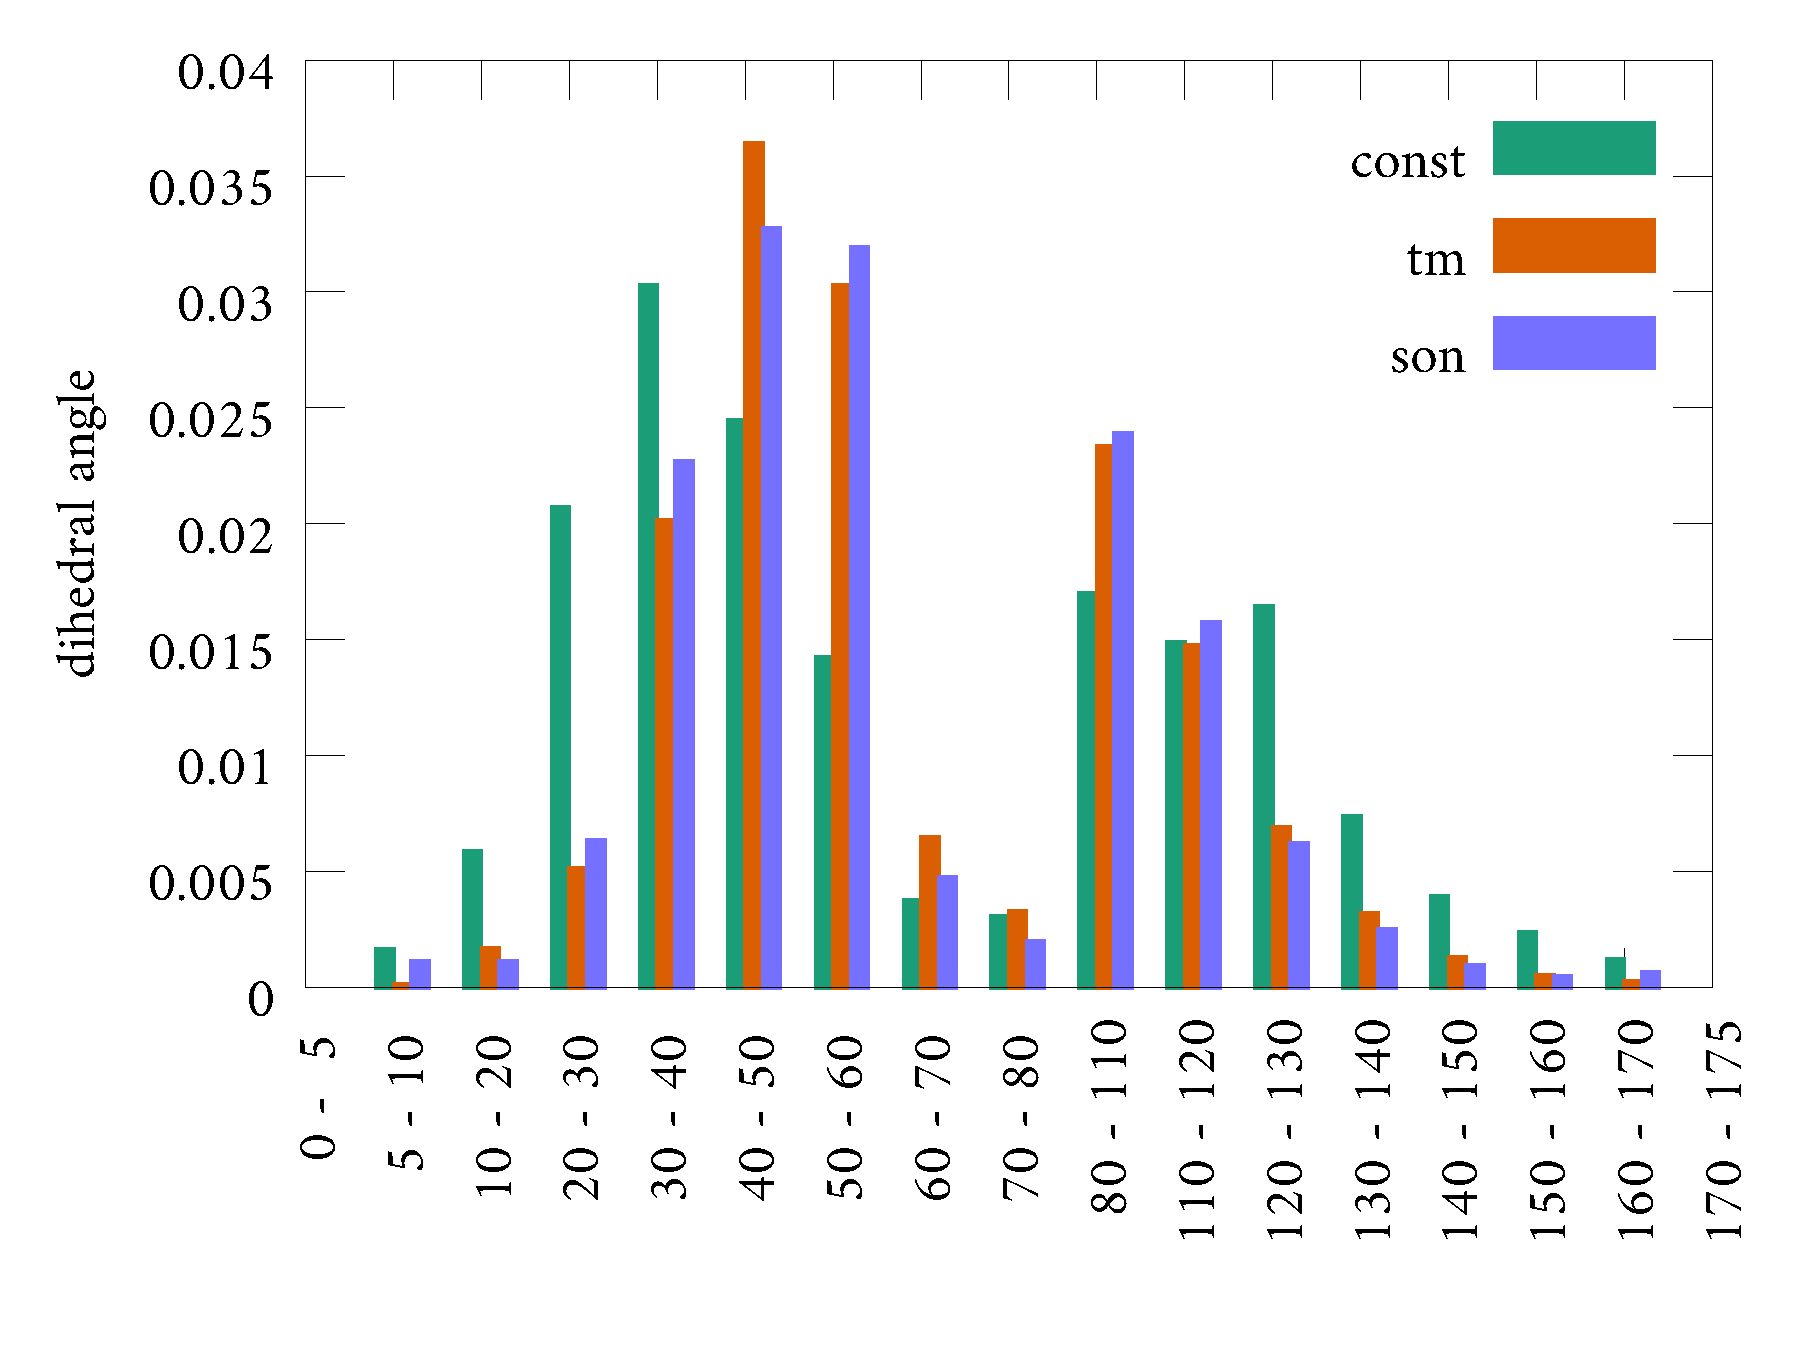
\includegraphics[width=\textwidth]{Figures/App/Rad_histAp2.pdf}
\end{subfigure}
\begin{subfigure}{0.5\textwidth}
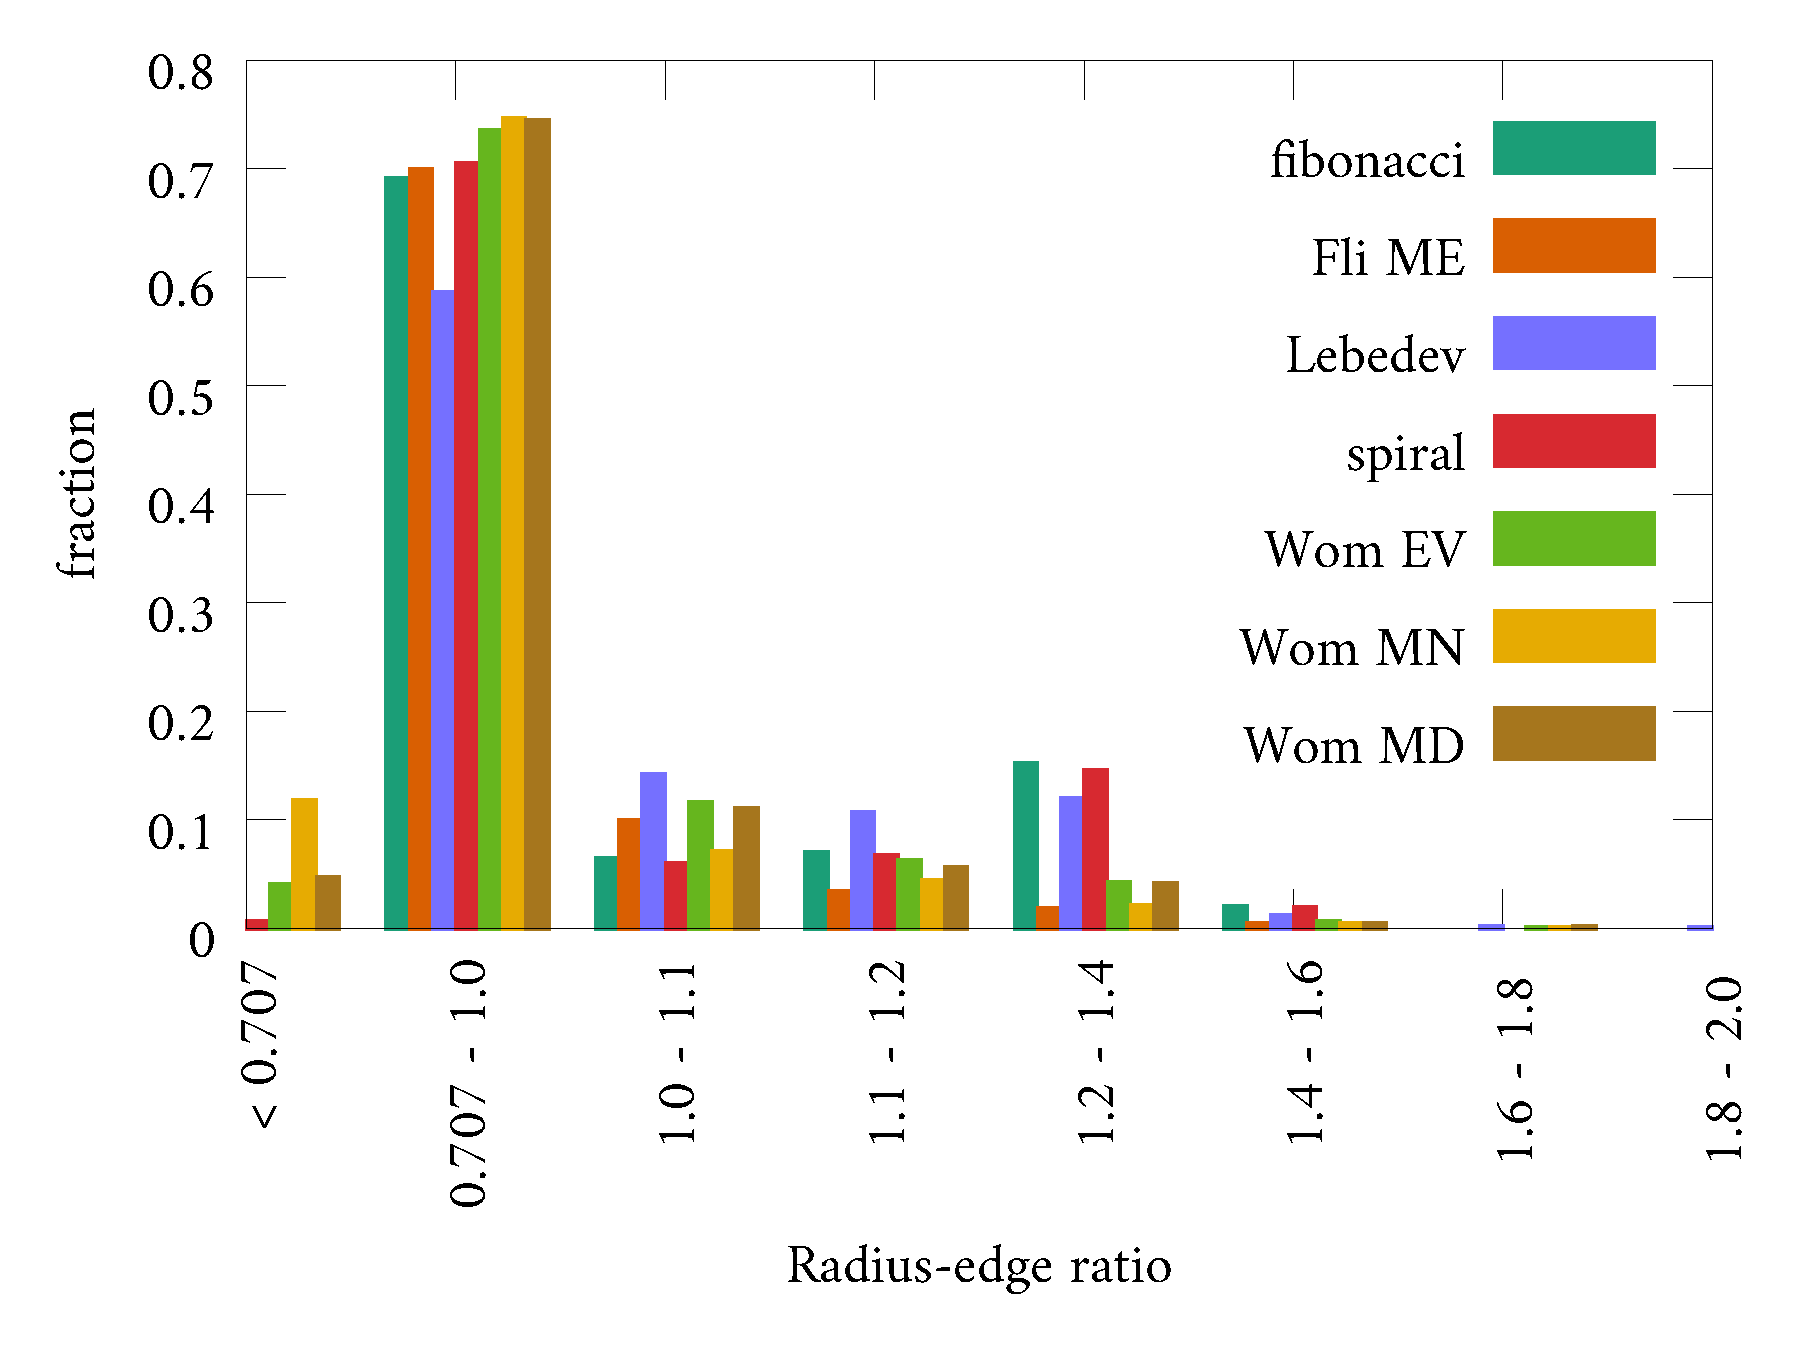
\includegraphics[width=\textwidth]{Figures/App/Sph_histAp1.pdf}
\end{subfigure}
\begin{subfigure}{0.5\textwidth}
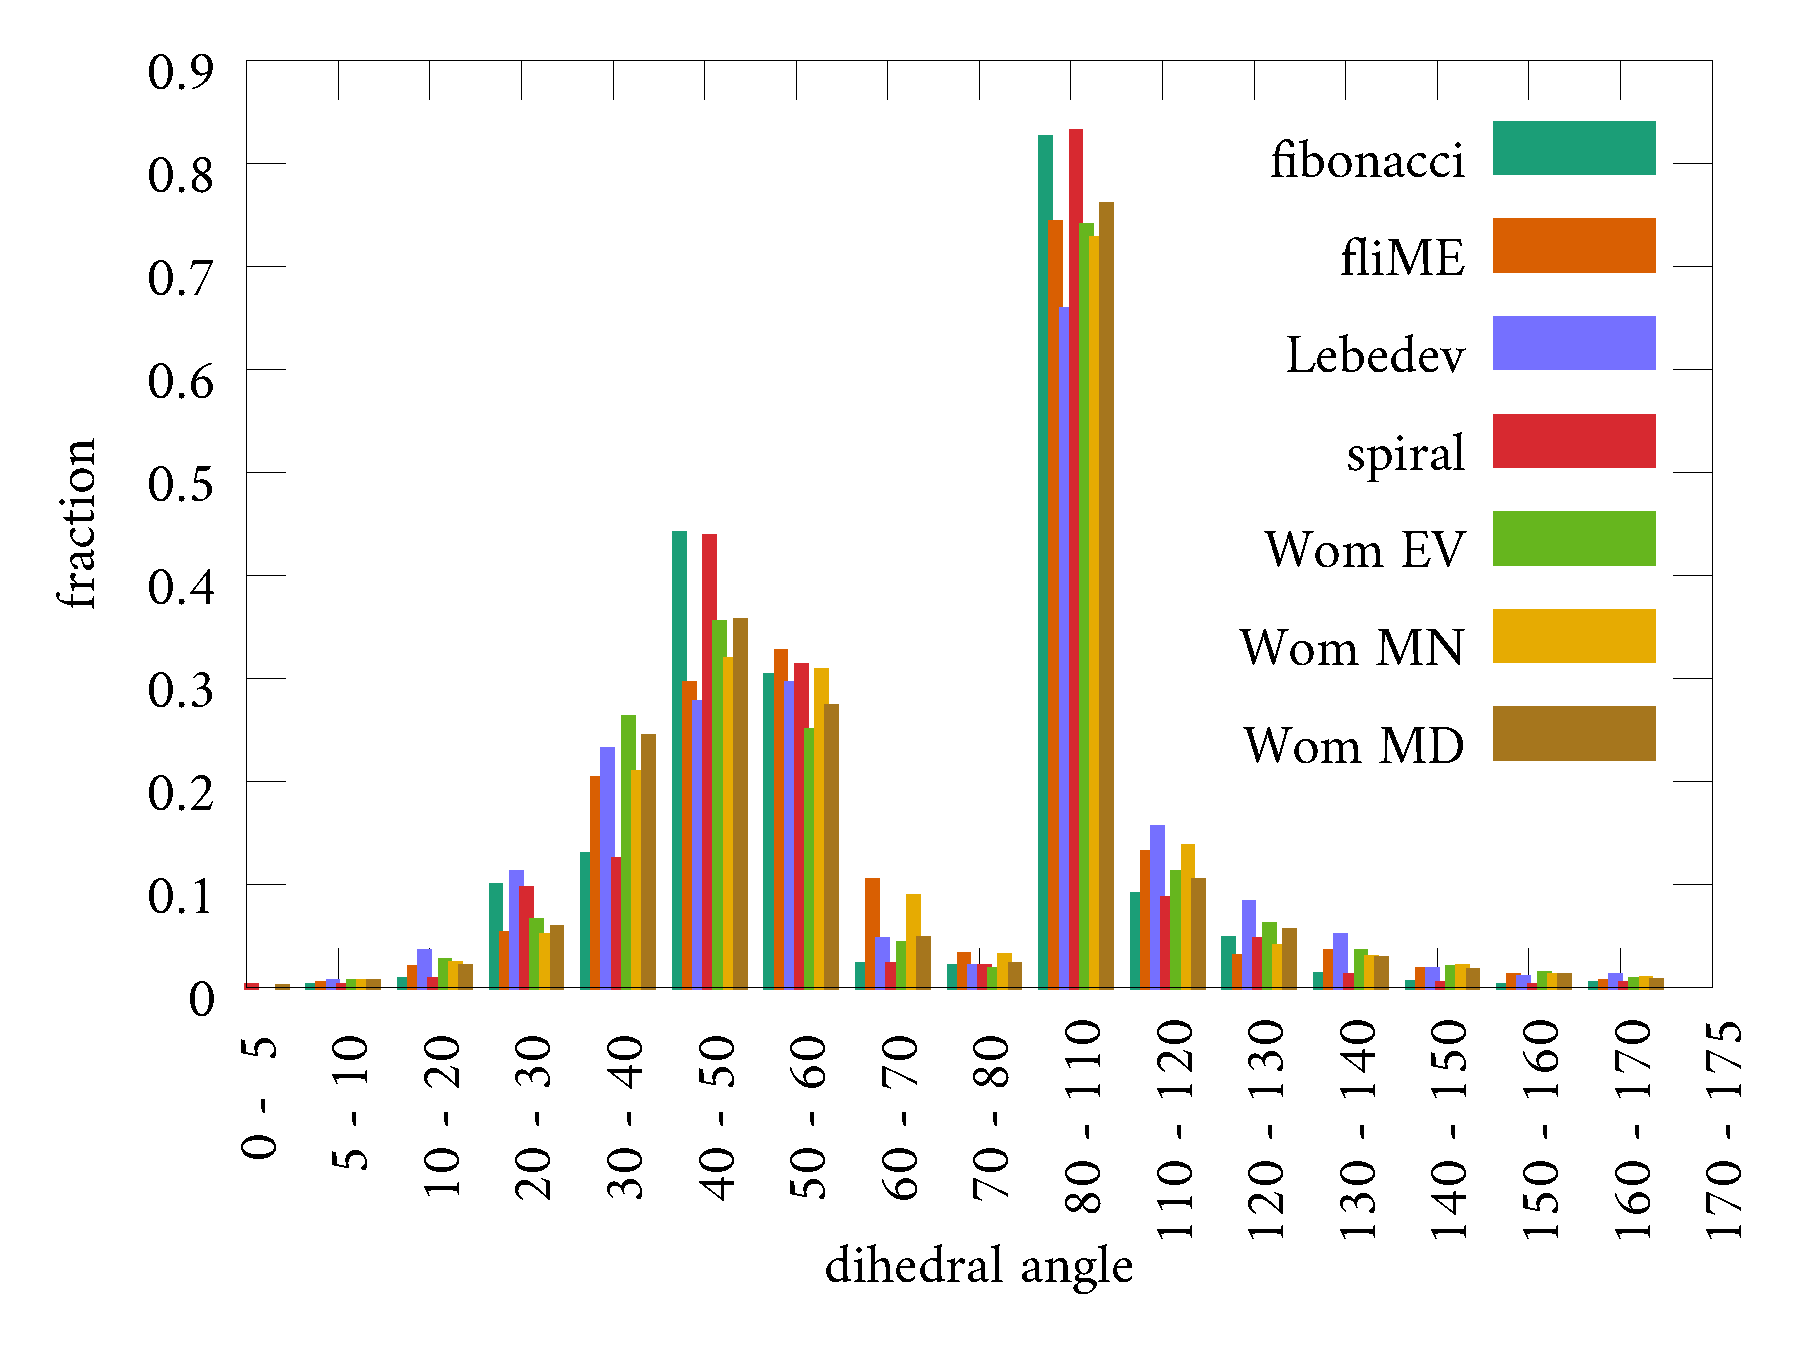
\includegraphics[width=\textwidth]{Figures/App/Sph_histAp2.pdf}
\end{subfigure}
\caption{Distribution of the ratio of radius and edge (left) and the dihedral angles (right)
for the different radial schemes (top) and angular distributions (bottom) described in section \ref{ch:GridSetup}.}
\label{appFig:SchemHist}
\end{figure}

%\begin{wrapfigure}{r}{0.7\textwidth}
\begin{figure}
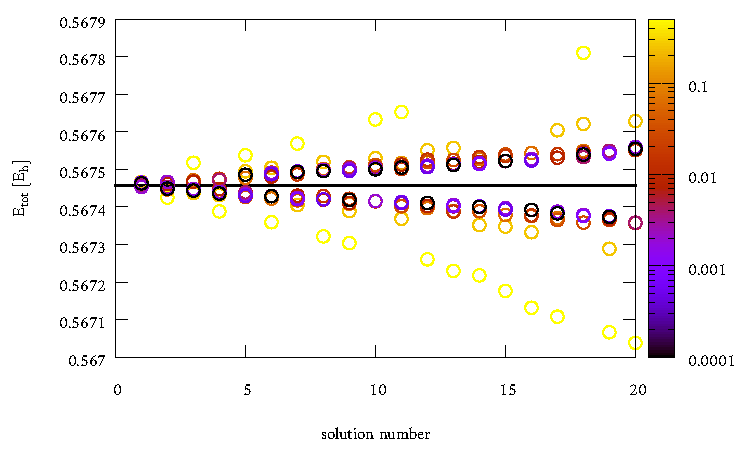
\includegraphics[width=0.7\textwidth]{Figures/IFem_powers_spectra}
\caption{The eigen energies of the first 20 solutions (circles) for different powers $p$ of the damping function $D(r)$ which determines the colours.
The spectra do not change significantly for $p<\frac 18$.}
\label{fig:powerSpect}
\end{figure}
%\end{wrapfigure}

%\subsection{Cross section}
%\begin{figure}
%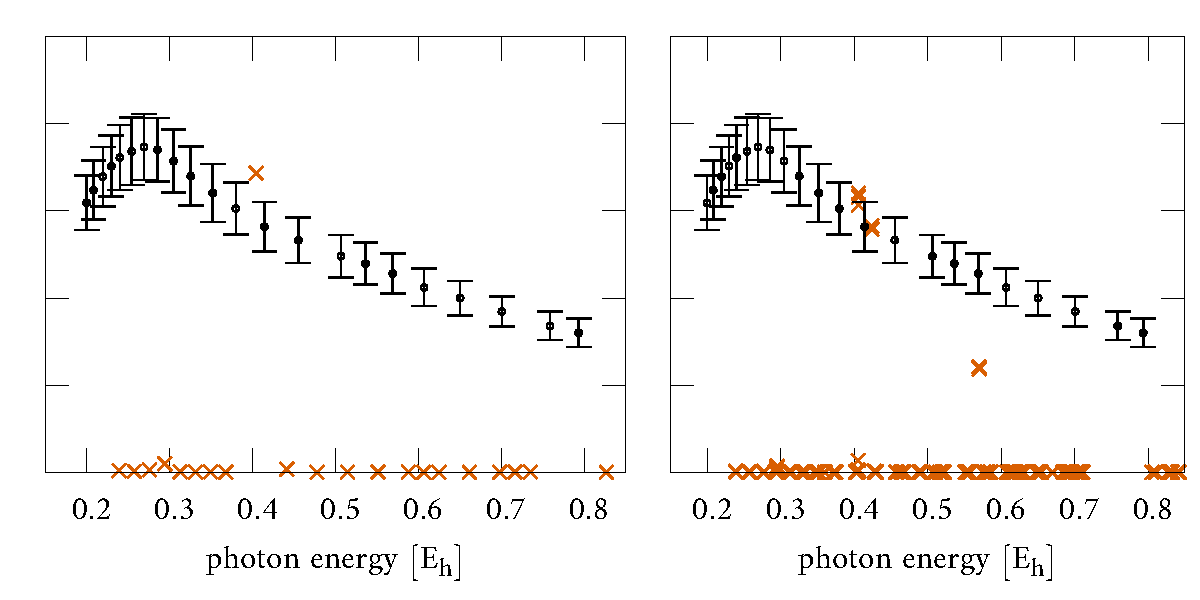
\includegraphics[width=\textwidth]{Figures/Lithium/CrossSectLB}
%\caption{Cross section of Lithium, obtained with a larger box.}
%\label{subfig:LiCS}
%\end{figure}
%
%\begin{figure}
%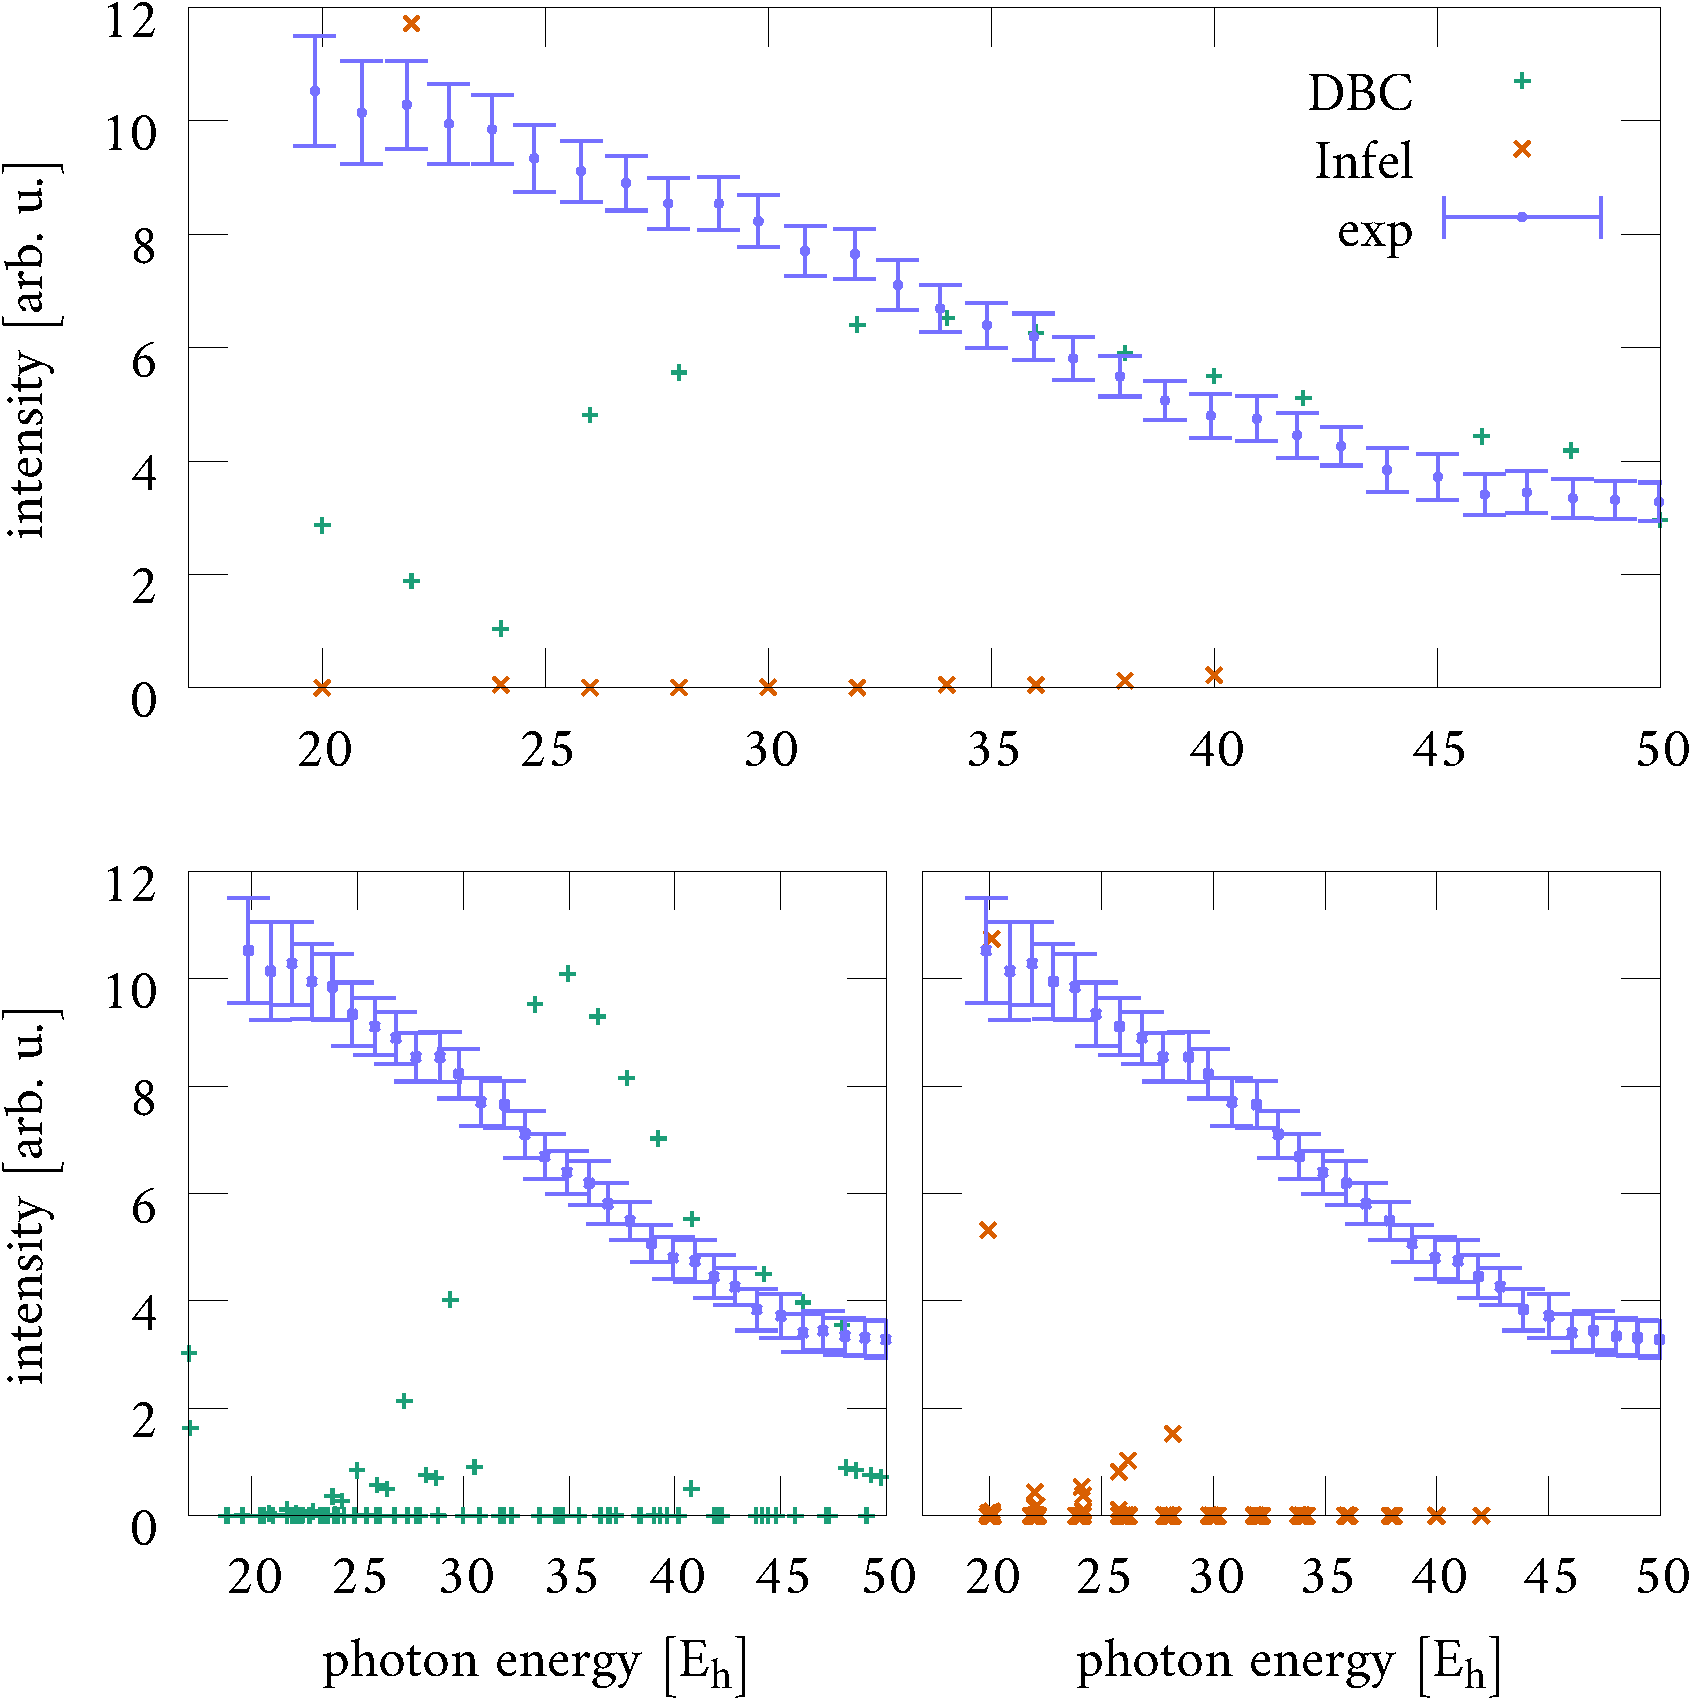
\includegraphics[width=\textwidth]{Figures/CO2/pi_uCS.pdf}
%\caption{Cross section of CO$_2$ for the $\pi_u$-transition.}
%\label{fig:piuCS}
%\end{figure}
%
%\subsection{Photoelectron spectra of Sulphur}
%\begin{figure}
   %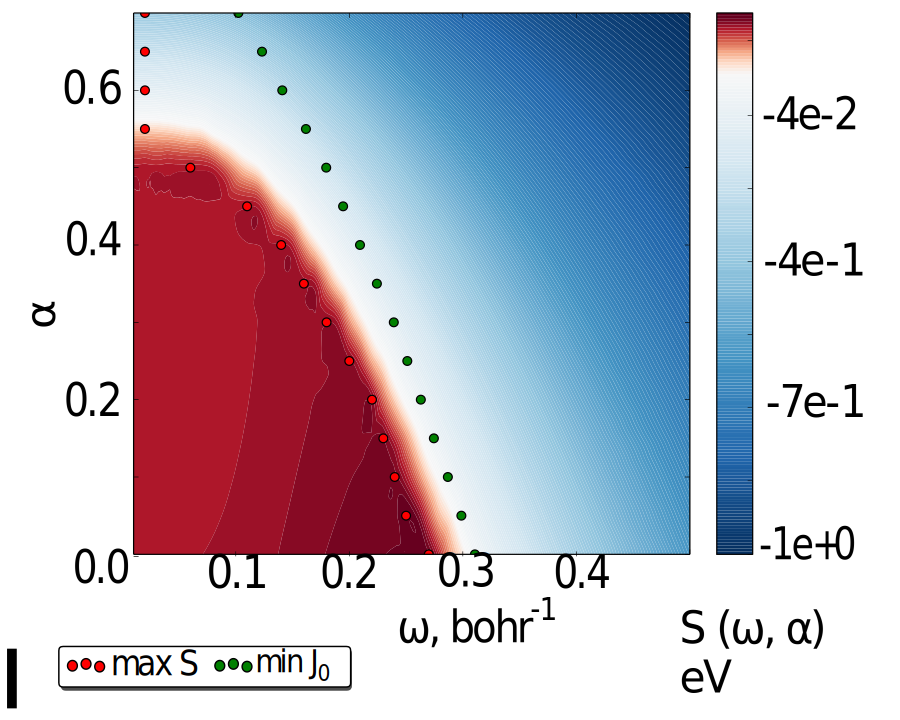
\includegraphics[width=\textwidth]{Figures/Sulphur/S8_stab_ion_cut_all}
   %\caption{deine Mudda}
   %\label{fig:SulphurStab}
%\end{figure}

%\begin{figure}
   %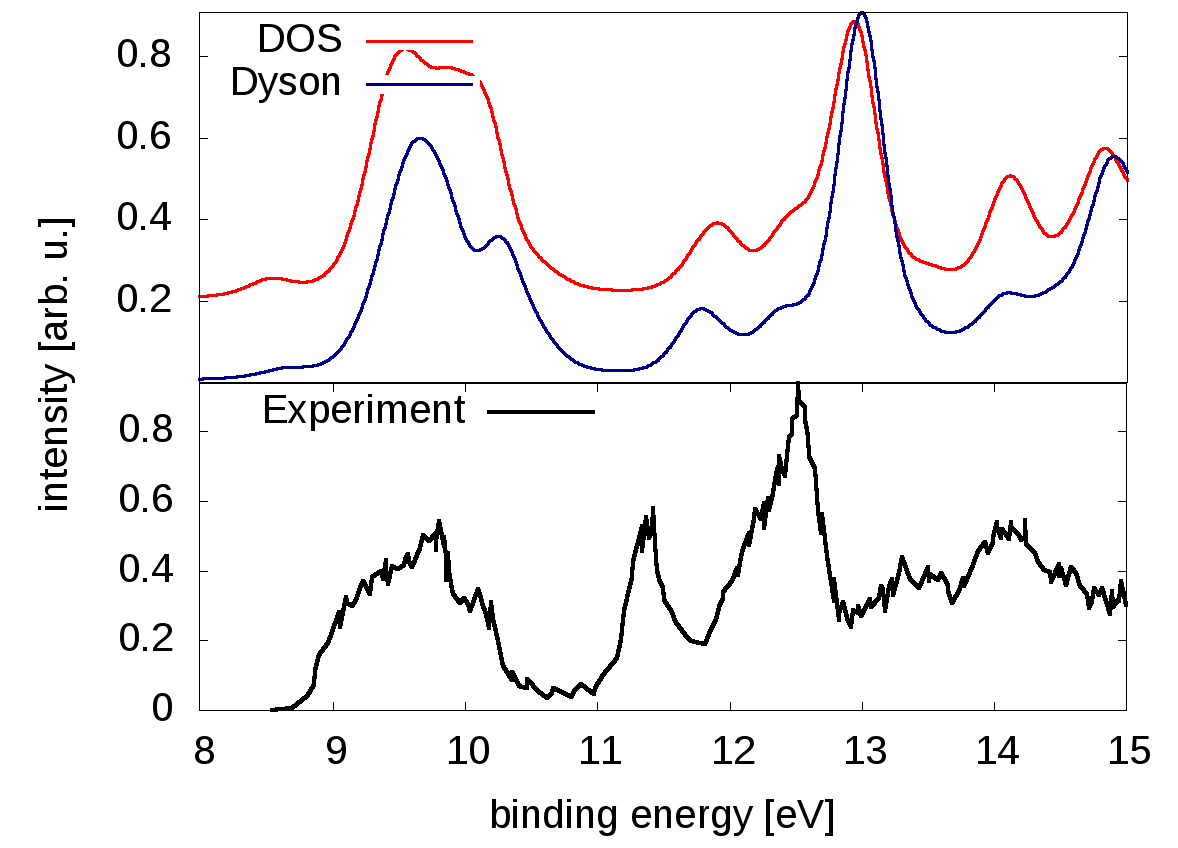
\includegraphics[width=\textwidth]{Figures/Sulphur/Sulphur}
%\end{figure}
%\begin{figure}
%\begin{subfigure}{0.5\textwidth}
   %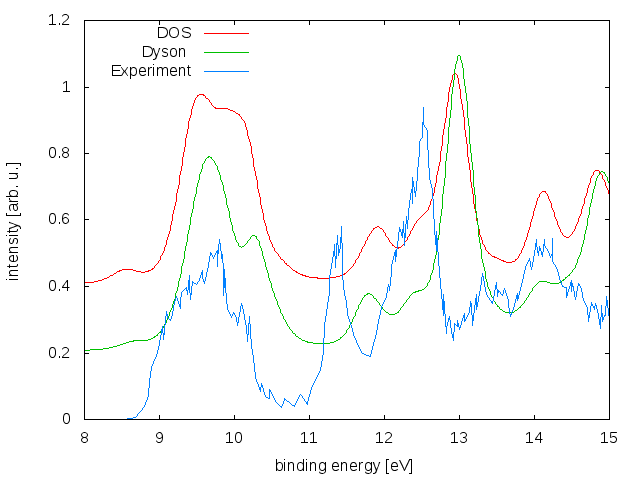
\includegraphics[width=\textwidth]{Figures/Sulphur/S8_vapour}
%\end{subfigure}
%\begin{subfigure}{0.5\textwidth}
   %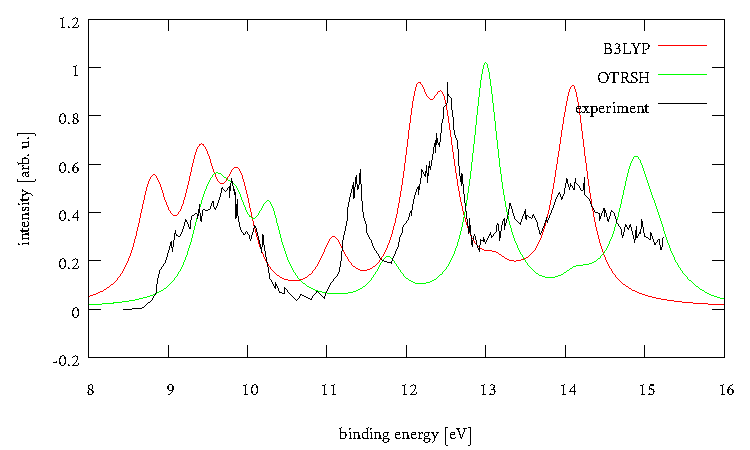
\includegraphics[width=\textwidth]{Figures/Sulphur/compS8}
%\end{subfigure}
%%\end{figure}
